\section{Task 2. A benchmark of configuration-dependent defects in configurable code}
\label{task2-section}

\subsection{Mine a large-scale corpus configuration-dependent defects}
\begin{figure}[h]
\centering
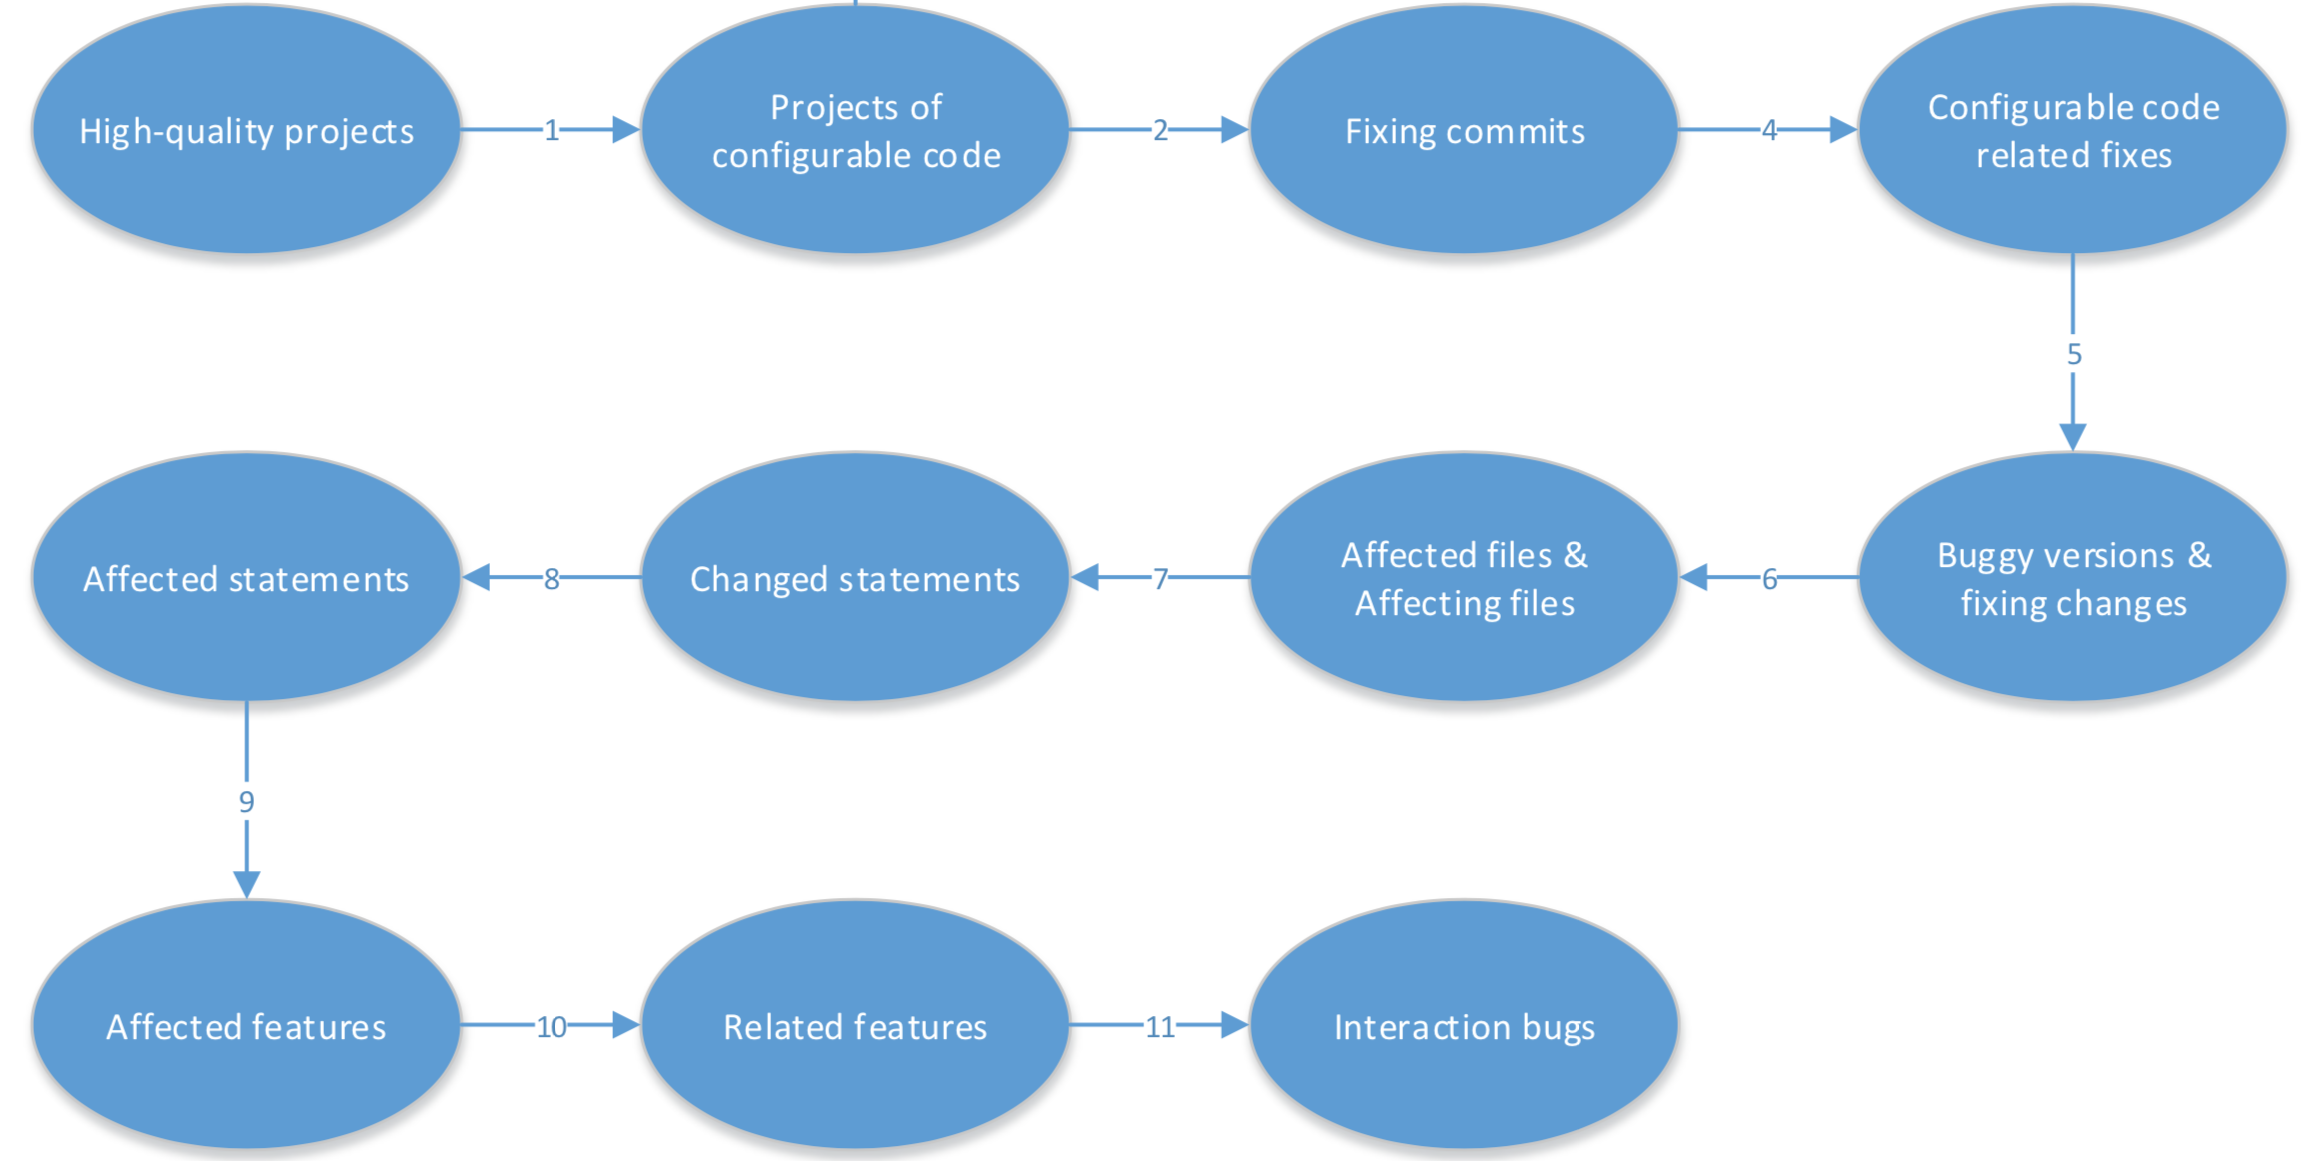
\includegraphics[width=0.8\textwidth]{benchmark}
\label{workflow}
\caption{An overview of configuration-dependent bugs mining}
\end{figure}
\begin{enumerate}
	\item Check if the current version of a project is configurable or not
	\item Extract fixing commits by patterns (e.g., containing words "fix", "error" or "bug")
	\item (Blank)
	\item Check if the changed files in the commit are configurable or included in any file of configurable code (accept if at least one of the changed files satisfy the condition). Note that check the inclusion of the file in the latest version and the intermediate version of the project.
	\item Checkout the buggy version and extract fixing changes
	\item Detect affected and affecting files (by inclusion). Also delete unrelated files
	\item Identify changed statements
	\item Identify the statements that are potentially affected by the changed
	\item Detect potential affected features. \textbf{If any feature is affected, then the version is a configuration-dependent bug}.
	\item Identify the features that are related (able to interact with) the affected features
	\item Extract the interaction information
	\item Manual check and record the conclusion
\end{enumerate}

\subsection{Preliminary results }